% - evaluation
% - conclusion

\section{Evaluation}
\begin{frame}{Instances}
    \begin{minipage}{0.6\textwidth}
        \centering
        \begin{tcolorbox}[colframe=black, colback=white, sharp corners=all, boxrule=0.5mm, boxsep=0mm, left=0mm, right=0mm, top=0mm, bottom=0mm]
            \begin{overpic}[width=\textwidth]{sparse/sparse_5_1.png}
                \put(5, 5){\textcolor{violet}{\textbf{Sparse}}}
            \end{overpic}
        \end{tcolorbox}
    \end{minipage}
    \begin{minipage}{0.1\textwidth}
    \end{minipage}
    \begin{minipage}{0.3\textwidth}
        \begin{minipage}{\textwidth}
            \centering
            \begin{tcolorbox}[colframe=black, colback=white, sharp corners=all, boxrule=0.5mm, boxsep=0mm, left=0mm, right=0mm, top=0mm, bottom=0mm]
                \begin{overpic}[width=\textwidth]{medium/medium_0_1.png}
                    \put(5, 5){\textcolor{violet}{\textbf{Medium}}}
                \end{overpic}
            \end{tcolorbox}
        \end{minipage}
        \begin{minipage}{\textwidth}
            \centering
            \begin{tcolorbox}[colframe=black, colback=white, sharp corners=all, boxrule=0.5mm, boxsep=0mm, left=0mm, right=0mm, top=0mm, bottom=0mm]
                \begin{overpic}[width=\textwidth]{dense/dense_0_1.png}
                    \put(5, 5){\textcolor{violet}{\textbf{Dense}}}
                \end{overpic}
            \end{tcolorbox}
        \end{minipage}
    \end{minipage}
\end{frame}

\begin{frame}{Instances - Details}
    \begin{minipage}{0.6\textwidth}
        \centering
        \begin{tcolorbox}[colframe=black, colback=white, sharp corners=all, boxrule=0.5mm, boxsep=0mm, left=0mm, right=0mm, top=0mm, bottom=0mm]
            \begin{overpic}[width=\textwidth]{sparse/sparse_5_1.png}
                \put(5, 5){\textcolor{violet}{\textbf{Sparse}}}
            \end{overpic}
        \end{tcolorbox}
    \end{minipage}%
    \begin{minipage}{0.4\textwidth}
        \begin{itemize}
            \item 3 domains
            \item 61 preselected instances (good estimates, no extreme edge cases, no haunted instances)
            \item increasing malfunctions
            \item singular connections between cities (to force problems)
        \end{itemize}
    \end{minipage}
\end{frame}

\begin{frame}{Testing}
    \begin{minipage}{0.6\textwidth}
        \centering
        \begin{overpic}[width=\textwidth]{benchmarking/sparse_rerun_cropped.eps}
            \put(5, 5){\textcolor{violet}{\footnotesize\textbf{Sparse}}}
        \end{overpic}
    \end{minipage}
    \begin{minipage}{0.1\textwidth}
    \end{minipage}
    \begin{minipage}{0.3\textwidth}
        \begin{minipage}{\textwidth}
            \centering
            \begin{overpic}[width=\textwidth]{benchmarking/medium_rerun_cropped.eps}
                \put(5, 5){\textcolor{violet}{\footnotesize\textbf{Medium}}}
            \end{overpic}
        \end{minipage}
        \begin{minipage}{\textwidth}
            \centering
            \begin{overpic}[width=\textwidth]{benchmarking/dense_rerun_cropped.eps}
                \put(5, 5){\textcolor{violet}{\footnotesize\textbf{Dense}}}
            \end{overpic}
        \end{minipage}
    \end{minipage}
\end{frame}

\begin{frame}{Testing - Worst Case Assumption}
    \begin{minipage}{0.6\textwidth}
        \centering
        \begin{overpic}[width=\textwidth]{benchmarking/sparse_rerun_cropped.eps}
            \put(5, 5){\textcolor{violet}{\footnotesize\textbf{Sparse}}}
        \end{overpic}
    \end{minipage}%
    \begin{minipage}{0.4\textwidth}
        \begin{itemize}
            \item less bad, than expected
            \item worst case assumption better in dense
        \end{itemize}
    \end{minipage}
\end{frame}

\begin{frame}{Testing - Reading vs Recomputation}
    \begin{minipage}{0.6\textwidth}
        \centering
        \begin{overpic}[width=\textwidth]{benchmarking/sparse_rerun_cropped.eps}
            \put(5, 5){\textcolor{violet}{\footnotesize\textbf{Sparse}}}
        \end{overpic}
    \end{minipage}%
    \begin{minipage}{0.4\textwidth}
        \begin{itemize}
            \item no meaningful difference between reading graph and computing graph
            \item slight favor for recomputation
        \end{itemize}
    \end{minipage}
\end{frame}

\begin{frame}{Testing - Instance in Detail}
    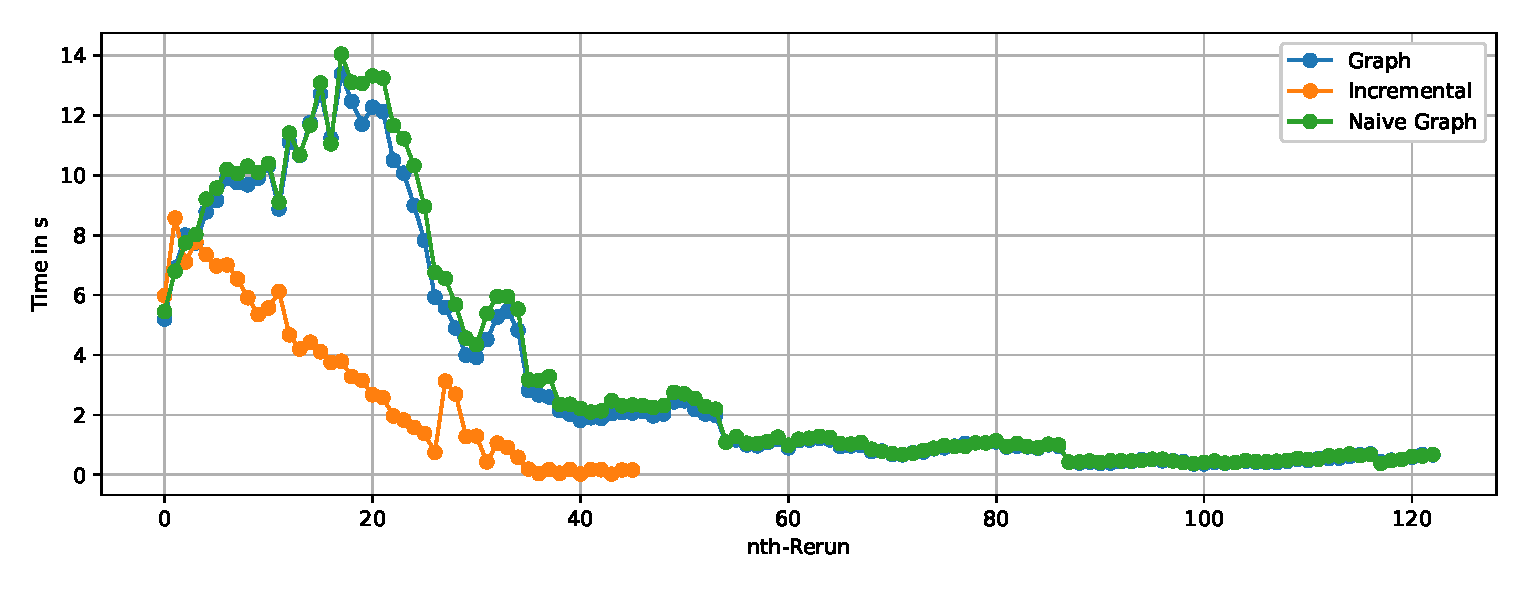
\includegraphics[width=0.9\textwidth]{benchmarking/medium_3_4_rerun_full.eps}
    \begin{minipage}{0.5\textwidth}
        Incremental
        \begin{itemize}
            \item peaks with additional timesteps
            \item continuously decreasing window
            \item shorter solution
        \end{itemize}
    \end{minipage}%
    \begin{minipage}{0.5\textwidth}
        Others
        \begin{itemize}
            \item increasing until trains despawn
            \item afterwards similar
            \item dangerous waiting
        \end{itemize}
    \end{minipage}
\end{frame}
 
\begin{frame}{Conclusions}
    \begin{itemize}
        \item incremental best, predicatable, adaptable, shorter paths
        \item negligible difference between reading and recalculating graph
        \item potential expansions
        \begin{itemize}
        \item pass grounding
        \item optimality
        \item resilient paths
        \end{itemize}
    \end{itemize}
\end{frame}